\documentclass[conference]{IEEEtran}
\IEEEoverridecommandlockouts

\usepackage[T1]{fontenc}
\usepackage[utf8]{inputenc}
\usepackage{cite}
\usepackage{amsmath,amssymb}
\usepackage{booktabs}
\usepackage{graphicx}
\graphicspath{{figures/}}
\usepackage{url}
\usepackage[hidelinks]{hyperref}

\begin{document}

\title{When Agentic Digital Twin Telemetry Measures Itself:\\
A Provenance Audit and a Gate}

\author{\IEEEauthorblockN{Umberto Altieri}
\IEEEauthorblockA{\textit{Independent Researcher}\\
\texttt{altieriumb7@gmail.com}}}

\maketitle

\begin{abstract}
Agentic Digital Twins delegate diagnostic and maintenance decisions to
tool-augmented language models, so predicting when such an agent is about to
fail---and abstaining---is a safety requirement. The signals proposed for this
are token-level uncertainty, verbalized confidence, and tool-execution
telemetry. We audited our own working pipeline, built to evaluate exactly those
signals on an industrial prognostics benchmark, and found that none of its
features measured the system they were taken to describe. Token logprobs were synthesised by
the logging layer from a hard-coded constant; verbalized confidence was never
elicited; the tool-error rate was inferred by substring-matching observation
text; the grading harness wrote its verdict into that same text; the telemetry
itself was re-derived by parsing run logs, inflating every structural feature;
and on $30$ of $75$ benchmark scenarios the tool layer fabricates the analytical
outcome, so the label records orchestration rather than prognostic accuracy.
Each defect is an ordinary engineering decision that produces a numerically
healthy column. We report six such defects with the cheap test that detects
each, release a gate that automates those tests and fails closed, and show what
the same analysis yields once the pipeline is repaired: on a re-collected corpus
of $225$ trajectories with provider-returned logprobs, early-step entropy
separates success from failure on two of three backbones
(AUROC $0.776$ and $0.746$) while the model's own post-hoc confidence does not
($0.494$), and the effect disappears entirely when backbones are pooled.
\end{abstract}

\begin{IEEEkeywords}
Digital Twin engineering, agentic systems, uncertainty quantification, data
provenance, reproducibility, predictive maintenance.
\end{IEEEkeywords}

\section{Introduction}

Industrial Digital Twins increasingly delegate work to LLM agents that
orchestrate diagnostic tools over standard interfaces~\cite{mcp}. Benchmarks in
this setting report that even strong backbones complete only around two thirds
of tasks~\cite{phmforge,assetops}. Because acting on a wrong prognosis costs far
more than deferring, a twin that recognises its own unreliable runs and abstains
is worth more than one that is merely more accurate. A model is calibrated when its stated confidence matches empirical
correctness~\cite{guo}; for agents the analogous question is
\emph{trajectory calibration}, predicting run success from signals observable
during execution of a ReAct-style loop~\cite{react}---token-level uncertainty~\cite{kadavath}, verbalized
confidence~\cite{xiong}, and execution telemetry~\cite{calvert}.

This paper is not about whether that works. It is about a prior question we did
not think to ask of our own pipeline: \emph{are these features measurements?}
For the pipeline we audited, none of them were. The defects are not exotic---a
fallback that keeps a long sweep running, a default for an unparsed field, a
status message appended to a trace---and each yields a column that passes every
check short of asking where the numbers came from.

\textbf{Relation to work on agent provenance.} A growing literature treats the
execution trace as the object of study, formalising it as a typed graph over
tool calls, memory accesses and retrieval steps in order to support
verification, debugging and accountability~\cite{provsurvey}, or auditing which
evidence a given action was actually conditioned on~\cite{provaudit}. That work
takes the trace as a faithful record and builds machinery on top of it. We
attack the prior assumption: the trace can be manufactured by the
instrumentation that writes it, and a provenance graph over a fabricated trace
inherits the fabrication without any inconsistency that graph-level analysis
would reveal. The checks we propose sit below that layer and ask whether each
recorded quantity was observed at all.

We contribute (i) six documented defects with a cheap detector for each,
(ii) a released gate that automates them and refuses a corpus that fails, and
(iii) a demonstration of what changes when the same analysis runs on repaired
instrumentation.

\section{Setting}
\label{sec:setting}

We state the setup explicitly, because the defects below are only visible once
one is precise about what is recorded and when.

A scenario is a natural-language maintenance request over a real asset dataset:
predict remaining useful life for every unit in a turbofan fleet, classify a
bearing fault, judge whether a maintenance window meets a safety policy. The
agent answers by interleaving a \emph{thought}, an \emph{action} naming a tool,
an \emph{action input}, and the \emph{observation} the tool returns, repeating
until it emits a terminating action or exhausts a step budget. A grader then
compares the final answer against scenario ground truth, yielding one binary
label per run. That sequence of steps, with the label, is a \emph{trajectory}.

Four families of features are extracted from it. \emph{Token} features summarise
the per-token log-probabilities of the agent's thoughts---their mean, their
variance, and the entropy of the first two steps. \emph{Verbalized} confidence is
the agent's own stated certainty. \emph{Structural} features describe the shape
of the trace: how many steps, how many tool calls, how often an action repeats,
whether it terminated properly. \emph{Error-rate} features count tool calls that
failed. The premise of trajectory calibration is that some combination of these
predicts the label well enough to support abstention.

Everything in this paper follows from asking where each of those numbers came
from.

\subsection{Why the twin needs this}

The asymmetry that makes calibration worth having is economic. Acting on a
prognosis that is wrong---scheduling no intervention on a component about to
fail---costs an unplanned outage. Deferring to a human engineer costs a review.
The two differ by orders of magnitude, so a twin that abstains on its least
reliable decisions converts the expensive error into the cheap one, even at
mediocre discrimination.

That argument only holds if the confidence estimate is real. A twin abstaining on
a signal that is actually a logging artifact does not reduce risk; it
redistributes it arbitrarily while appearing instrumented, which is worse than
having no abstention at all, because the operator now trusts a control that does
nothing. This is why provenance is a safety property here rather than a matter
of experimental hygiene.

\section{Six Provenance Defects}
\label{sec:defects}

The audited pipeline evaluates five calibration schemes over $167$ trajectories
from seven backbones on PHMForge~\cite{phmforge}. Illegitimate features are a
leading cause of irreproducibility in ML-based science~\cite{kapoor}; what
follows is that failure mode arising from agent instrumentation rather than from
dataset construction. Table~\ref{tab:defects}
summarises what each of its feature families actually contained.

\begin{table}[t]
\centering
\caption{Defects found, the evidence, and the test that detects each. Every
value in every column was individually well-formed.}
\label{tab:defects}
\footnotesize
\begin{tabular}{p{1.45cm}p{3.1cm}p{2.6cm}}
\toprule
\textbf{Defect} & \textbf{Evidence} & \textbf{Detector} \\
\midrule
Logprobs synthesised & All $203{,}107$ tokens fit the logger's own fallback
generator $\mathcal{N}(-0.40,0.225^2)$; observed $-0.4030\pm0.2182$ &
Compare moments against what the fallback would emit \\
\addlinespace
Confidence never elicited & $162/167$ trajectories carry a hard-coded $0.75$;
parsed once per run, so its gradient is $0$ by construction &
Count distinct values; a constant cannot inform \\
\addlinespace
Error rate is prose, not protocol & \texttt{status\_code} set by matching
``Error''/``failed'' in observation text; no response metadata is read &
Require the status the tool server returned \\
\addlinespace
Grader verdict leaks & Terminal observation reads ``Task finished
successfully''/``Task failed''; the \emph{only} observation for $71$ single-step
runs & Non-monotone learner far above a feature's univariate AUROC \\
\addlinespace
Telemetry reconstructed & Re-derived by parsing logs; the single-use
\texttt{Finish} appears $866$ times, $790$ mid-trajectory &
Check trace shape against what the agent can emit \\
\addlinespace
Label fabricated & \texttt{predict\_rul} returns ground truth plus
$\mathcal{N}(-3,14^2)$ at fixed seed, giving MAE $9.01$ inside the grader's
$[7,18]$ window; \texttt{classify\_faults} invents its ground truth too &
Read the tool, not its output \\
\bottomrule
\end{tabular}
\end{table}

\begin{figure}[t]
\centering
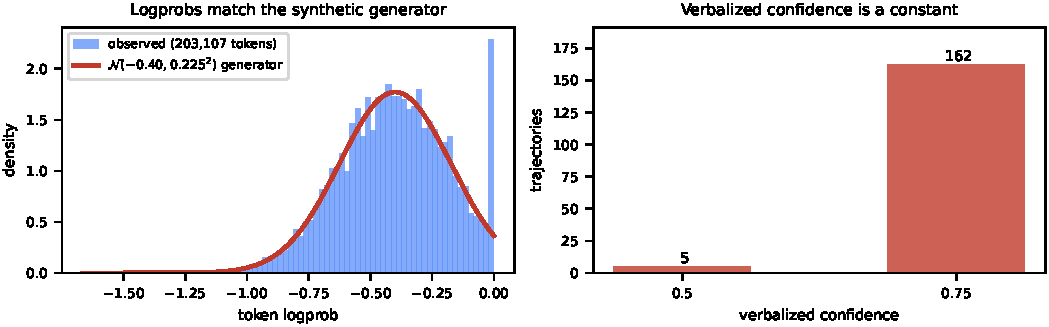
\includegraphics[width=\columnwidth]{figures/fig2_provenance.pdf}
\caption{Provenance evidence. \textbf{Left:} all $203{,}107$ logged token
logprobs against the density of the logging layer's own fallback generator at
its default confidence. The fit is exact; the spike at zero is the generator's
clipping. \textbf{Right:} verbalized confidence takes one value on $162$ of
$167$ trajectories. Neither family was obtained from a model.}
\label{fig:prov}
\end{figure}

Fig.~\ref{fig:prov} shows the two clearest cases. The test that produced it is
one line---compare the empirical moments of a generation-derived feature against
what the fallback path would emit---and it is the cheapest guard we know of
against an uncertainty feature that is not a measurement.

Three points generalise beyond this codebase. First, the logprob chain was
broken in \emph{four} independent places---the client never requested them, one
of two agent classes discarded them, the default serialisation branch omitted
them, and the logger synthesised a replacement. Fixing any three would have
changed nothing observable, because the fourth still supplied plausible numbers.
That is how a fabricated feature survives review: the defect is distributed
across individually reasonable layers, and the fallback removes the error signal
that would force someone to look.

Second, the last defect concerns the \emph{target}, and no feature audit could
have found it. Every column can be a perfect measurement while the quantity
being predicted is not the one of interest. It is worth seeing directly. The
tool that is supposed to run the trained model instead does this:

\begin{verbatim}
gt = load_rul_ground_truth(fd)
rng = np.random.default_rng(seed=42)
shifts = rng.normal(loc=-3.0, scale=14.0, size=n)
preds = [max(0.0, round(g + s, 2))
         for g, s in zip(gt, shifts)]
\end{verbatim}

The trained model is loaded and the result discarded. Predictions are ground
truth plus noise at a fixed seed, and the noise is tuned---the docstring says
so---to land the downstream error metrics inside the range the grader accepts.
Success on those scenarios therefore records whether the agent called the tools
in a workable order and reported what they returned. It records nothing about
prognostic accuracy, which belongs to the generator.

Third, we did not repair the benchmark. Modifying a benchmark's tools forfeits
comparability with everything published on it. We instead use the split as a
design: $45$ scenarios whose tools compute deterministically from what the agent
supplies, and $30$ whose outcome is fabricated.

\section{A Gate That Fails Closed}

We release a provenance gate that runs before any modelling and exits non-zero
when no measured signal family survives. Four checks correspond to the defects
above: constant columns, distributions matching a fallback generator,
harness verdict strings in fields features can reach, and columns flagged
unmeasured. The synthetic-logprob test is not tuned to one generator: it keys on
three properties real logprobs have---strong negative skew, poor Gaussian fit,
and non-trivial mass above $-0.01$. Measured on the original corpus these read
$-0.20$ and $4.3\%$; on repaired instrumentation, $-5.15$ and $86.8\%$.

Two further checks came from failures of the repaired pipeline, and are the ones
we would most want others to adopt.

\textbf{Degenerate trajectories.} A run recording no extracted action is a
failed collection, not a hard instance. A provider that refuses by returning an
empty generation is indistinguishable from a weak model: the agent parses
nothing, exhausts its step budget on format errors, and writes an
ordinary-looking failure. This destroyed $200$ of $225$ trajectories in one of
our runs, at a tenth of the normal wall time.

\textbf{Availability leakage.} Provenance asks whether each recorded value is a
measurement. It cannot see the case where every value is genuine but the rows
carrying the column are also the rows that succeed---then a model separates the
classes by detecting its own availability, and the imputation filling the gap
becomes the signal. In the run above, token features survived on $25$ of $225$
trajectories and all $11$ successes lay inside them; every family scored above
$0.9$ AUROC while measuring only which runs had been collected. The gate now
compares outcome rates on rows that have a column against those that do not.

A self-test builds one honestly captured corpus and one reproducing the defects
of Sec.~\ref{sec:defects}, and asserts the gate accepts the first and rejects
the second.

\section{What Changes When the Features Are Real}

To ask the original question at all we repaired the instrumentation and
re-collected. This required leaving the managed inference gateway entirely: it
refuses the logprobs parameter on every open-weights model it hosts---verified
on five, on both its endpoints, as a warning rather than an error, so the call
succeeds and the field is silently absent. Only its commercial model returns
them. That is an awkward constraint for a field whose deployments are the least
able to use a commercial API, and it means token-level uncertainty is
unobservable on gateway-hosted open weights.

We re-ran all $75$ scenarios on three open-weights backbones served over an
OpenAI-compatible API: $225$ trajectories, Pass@1 $0.556$, one degenerate run,
gate-certified. Table~\ref{tab:res} reports the computed-outcome stratum.

\begin{table}[t]
\centering
\caption{Out-of-fold AUROC on the $45$ scenarios whose outcome the tools
actually compute, per backbone ($n=45$ each). $^{\ast}$ significant at the
Bonferroni threshold over all $15$ comparisons ($\alpha=0.0033$).}
\label{tab:res}
\footnotesize
\begin{tabular}{lccc}
\toprule
\textbf{Signal} & \textbf{qwen2.5-7b} & \textbf{llama-3.3-70b} & \textbf{gpt-oss-120b} \\
\midrule
Early-step entropy & $\mathbf{0.776}^{\ast}$ & $0.539$ & $\mathbf{0.746}^{\ast}$ \\
Structural         & $0.648$ & $0.547$ & $0.441$ \\
Observation        & $0.664$ & $0.589$ & $0.312$ \\
Self-reported conf.& $0.494$ & $0.577$ & $0.421$ \\
\midrule
\textit{Pooled, 3 backbones} & \multicolumn{3}{c}{\textit{$0.517$--$0.567$, none significant}} \\
\bottomrule
\end{tabular}
\end{table}

Three observations. \textbf{Token uncertainty separates on two backbones of
three}, at AUROC $0.776$ and $0.746$, surviving correction over all comparisons
made. Out-of-fold permutation importance---preferred to impurity-based measures,
which are biased toward high-cardinality continuous
predictors~\cite{strobl}---attributes essentially all of it to the entropy of
the first two steps; variance over the whole trajectory contributes nothing.
Operationally that favours abstaining after two steps rather than executing a
full trajectory and discarding it.

\textbf{The model's own confidence does not separate} ($0.494$ on the backbone
where entropy scores $0.776$). We elicited it post hoc, from the model that
produced each trajectory, because asking in band made models over-generate past
the action input, corrupting the tool argument and driving Pass@1 to zero. The
elicited values are well dispersed ($9$ distinct values, $\sigma=0.36$), so this
is a discriminating baseline that discriminates poorly---not a degenerate one.

\textbf{Pooling destroys the effect.} Features identify the generating backbone
in $92\%$ of rows, so mixing three populations makes the rankings
incommensurable: a logprob that is low for one model is not low in the same way
for another. Trajectory calibration appears to be a per-model exercise.

\section{Checklist, Limitations, Availability}

Beyond the six detectors, four checks cost little and would have caught most of
what we found.

\textbf{Declare provenance per feature.} State for each column whether it is
provider-returned, parsed, derived, or imputed, and report the imputation rate.
A column imputed on every row is not evidence, whatever its distribution looks
like.

\textbf{Reconcile runs attempted against runs recorded.} Count them separately
and require them to match. No inspection of values can find a missing row,
because the surviving rows are individually valid; a loop that logs only what it
wrote reports complete success while discarding cases. An encoding error on
agent output cost us $44\%$ of one run, selectively, and the survivors looked
healthier than the full set.

\textbf{Verify the provider answered, not that the call returned.} Refusal need
not raise. Treat runs that finish implausibly fast as suspect, and probe each
backbone for a non-empty generation carrying the fields the study depends on
before collecting anything.

\textbf{Group folds by scenario, and report both trivial policies.} Multi-backbone
sweeps over a shared scenario set leak across models otherwise. And a selective
method must be compared against always-abstain as well as always-execute: in the
original study the ``optimised'' policy was twice as expensive as abstaining on
everything, which no reported number revealed because that baseline was never
computed.

\textbf{Limitations.} The detectors were derived from one pipeline and validated
against synthetic fixtures, not against independently authored corpora. Whether
these six defects recur elsewhere, or are idiosyncratic to this codebase, we
cannot answer from a sample of one; what the case establishes is that each is
reachable by ordinary engineering decisions and invisible to value-level
inspection, which is a claim about the class rather than its frequency.

The empirical section illustrates rather than establishes.
Each cell holds $n=45$, with intervals near $\pm0.16$; two of three backbones
show the effect and we cannot explain the third; all three are quantised
variants from one provider; and the significant cells were found after exploring
fifteen comparisons, so they warrant confirmation on fresh runs rather than
treatment as settled. The audit findings in Sec.~\ref{sec:defects} carry no such
caveat---they are demonstrations, not estimates.

Code, gate, telemetry, and the harness that reproduces every number:
\url{https://github.com/altieriumb7/trajectory-calibration-digital-twins}.

\begin{thebibliography}{99}
\bibitem{mcp} Anthropic, ``Model Context Protocol specification,'' 2024.
[Online]. Available: \url{https://modelcontextprotocol.io}
\bibitem{phmforge} T. Feng \emph{et al.}, ``PHMForge: Evaluating LLM agents on
industrial prognostics through MCP-native, algorithm-grounded tools,''
\emph{arXiv:2604.01532}, 2026.
\bibitem{assetops} D. Patel \emph{et al.}, ``AssetOpsBench: Benchmarking AI
agents for task automation in industrial asset operations and maintenance,''
\emph{arXiv:2506.03828}, 2025.
\bibitem{react} S. Yao \emph{et al.}, ``ReAct: Synergizing reasoning and acting
in language models,'' in \emph{Proc. ICLR}, 2023.
\bibitem{kadavath} S. Kadavath \emph{et al.}, ``Language models (mostly) know
what they know,'' \emph{arXiv:2207.05221}, 2022.
\bibitem{xiong} M. Xiong \emph{et al.}, ``Can LLMs express their uncertainty? An
empirical evaluation of confidence elicitation in LLMs,'' in \emph{Proc. ICLR},
2024.
\bibitem{calvert} A. Vinod, Y. Ding, and E. Stengel-Eskin, ``CalVerT:
Augmenting agents with calibrated verifier telemetry improves action and
learning in knowledge-intensive tasks,'' \emph{arXiv:2606.21777}, 2026.
\bibitem{guo} C. Guo, G. Pleiss, Y. Sun, and K. Q. Weinberger, ``On calibration
of modern neural networks,'' in \emph{Proc. ICML}, 2017.
\bibitem{strobl} C. Strobl, A.-L. Boulesteix, A. Zeileis, and T. Hothorn,
``Bias in random forest variable importance measures,'' \emph{BMC
Bioinformatics}, vol. 8, no. 25, 2007.
\bibitem{kapoor} S. Kapoor and A. Narayanan, ``Leakage and the reproducibility
crisis in machine-learning-based science,'' \emph{Patterns}, vol. 4, no. 9,
2023.
\bibitem{provsurvey} Y. Wang \emph{et al.}, ``From agent traces to trust: A
survey of evidence tracing and execution provenance in LLM agents,''
\emph{arXiv:2606.04990}, 2026.
\bibitem{provaudit} J. Liao, ``Auditing provenance sensitivity in LLM agent
action selection,'' \emph{arXiv:2607.20827}, 2026.
\end{thebibliography}

\end{document}
